\documentclass{beamer}

% To have the citation lists ordered by number.
\usepackage[nocompress]{cite}
\usepackage[utf8]{inputenc}
\usepackage{graphicx}
\usepackage[tight,TABTOPCAP]{subfigure}
\usepackage{amsmath}
\usepackage{amssymb}
\usepackage{amsfonts}
\usepackage{url}

\usepackage{hyperref}

\usepackage{tikz}
\usepackage{color}

% Allow more than 70% (default) of a page to be filled by figures (100%).
\renewcommand\topfraction{1.0}

%%%%%%%%%% Tool Names %%%%%%%%%%%%
\newcommand{\csisat}{{\sc CSIsat}}
\newcommand{\blast}{{\sc Blast}}
\newcommand{\armc}{{\sc ARMC}}
\newcommand{\mathsat}{{\sc MathSAT}}
\newcommand{\picosat}{{\sc PicoSAT}}
\newcommand{\clpprover}{{\sc CLPprover}}
\newcommand{\foci}{{\sc Foci}}
\newcommand{\sicstus}{{\sc SICStus Prolog}}


%%%%%%%%%% NOTATIONS %%%%%%%%%%%%
\newcommand{\true}{{\it true}}
\newcommand{\false}{{\it false}}
\newcommand{\sat}{{\sc sat}}
\newcommand{\laeuf}{{\sc LA+EUF}}

\renewcommand{\implies}{\Rightarrow}


\hyphenation{CEGAR Blast sicstus prolog clpprover}

%TODO explain what is the CSIsat acronym ?
%DONE Craig citation
%DONE foci citation
%DONE clp citation
%DONE blast citation
%DONE slide number
%DONE name color (italic)
%DONE performance slide
%DONE related work MathSat
% inductive interpolant (Gregory), not needed (Tom)
%DONE syntax (infix)
%TODO application slide


\mode<presentation>
{
  \usetheme{Warsaw}
  %\usetheme{Frankfurt}
  % or ...

  %\setbeamercovered{transparent}
  % or whatever (possibly just delete it)
  %\setbeamertemplate{footline}[frame number]
  \useoutertheme{mysplit}
}
% Remove the navigation bar
\setbeamertemplate{navigation symbols}{}

\graphicspath{{./imgs/}}

\title[\csisat{}]{\csisat{}: Interpolation for \laeuf{}}

\AtBeginSection[]
{
  \begin{frame}<beamer>
    \frametitle{Outline}
    \tableofcontents[currentsection]
  \end{frame}
}

\author{Dirk Beyer\inst{1}     
\and 
        \textbf{Damien Zufferey}\inst{2}
%        \textcolor{blue}{Damien Zufferey}\inst{2}
\and 
        Rupak Majumdar\inst{3} 
}

\institute{
  ${}^1$ Simon Fraser University, BC, Canada \and
  ${}^2$ EPFL, Switzerland \and
  ${}^3$ UCLA, CA, USA   
}
\date{\vspace{5mm}\\ CAV'08, Princeton, ~~ July 11, 2008}

%-------------------------------------------------------------------------
\begin{document}

% Title
\frame[plain]{\titlepage}

\section*{Outline}
\begin{frame}
\tableofcontents
\end{frame}

\section{Interpolation}
\begin{frame}
  \frametitle{Definition [Craig 57]}
  Let $A$ and $B$ be two formulas such that
  $A \wedge B$ unsat.\\
  An interpolant $I$ has the following properties:
  \begin{itemize}
  \item $I$ contains only $AB$-common symbols.
  \item $A$ implies $I$
  \item $I \wedge B$ unsat.
  \end{itemize}
  Interpolation exists for $\text{\laeuf{}}$.
\end{frame}

\begin{frame}
%TODO b not in B
  \frametitle{Interpolant for EUF}
  \textcolor{blue}{$A$: ~~ $a = b \wedge b = c$} \hfill
  \textcolor{red}{$B$: ~~ $f(a) \ne f(c)$}
  \begin{figure}
  \centering
  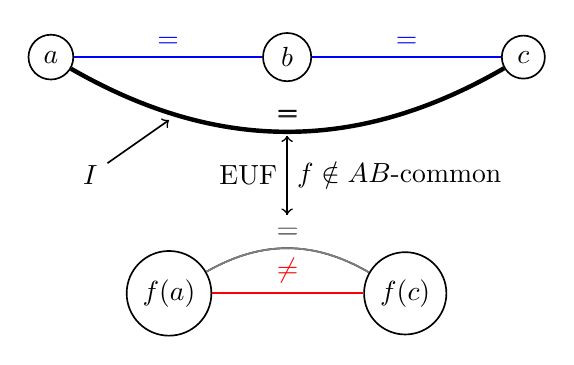
\begin{tikzpicture}[auto, node distance=3cm, semithick]
  \node [circle,draw] (a) at (0,3) {$a$};
  \node [circle,draw] (b) [right of=a] {$b$};
  \node [circle,draw] (c) [right of=b] {$c$};
  \node [circle,draw] (f_a) at (1.5,0) {$f(a)$};
  \node [circle,draw] (f_c) [right of=f_a] {$f(c)$};
  \path [draw=blue] (a) edge node {\textcolor{blue}{$=$}} (b);
  \path [draw=blue] (b) edge node {\textcolor{blue}{$=$}} (c);
  \path [draw=red] (f_a) edge node {\textcolor{red}{$\ne$}} (f_c);
  \visible<2-4>{\path (a) edge [bend right] node {$=$} (c);}
  \visible<3>{\path (f_a) edge [bend left] node {$=$} (f_c);}
  \visible<4->{\path [draw=gray] (f_a) edge [bend left] node {\textcolor{gray}{$=$}} (f_c);}
  \visible<3>{\draw [->] (3,2) to node[left] {EUF} (3,1);}
  \visible<4>{\draw [->] (3,1) to node[right] {$f \notin AB$-common} (3,2);}
  \visible<5->{
    \path [ultra thick] (a) edge [bend right] node {$=$} (c);
    \node [draw=none] (i) at (0.5,1.5) {$I$};
    \draw [->] (i) to (1.5,2.2);
  }

  \end{tikzpicture}
  \end{figure}
\end{frame}

\begin{frame}
  \frametitle{Interpolant for LA}
  \textcolor{blue}{$A \vec{x} \leq \vec{a}$} \hfill
  \textcolor{red}{$B \vec{x} \leq  \vec{b}$}
  \begin{figure}
  \centering
  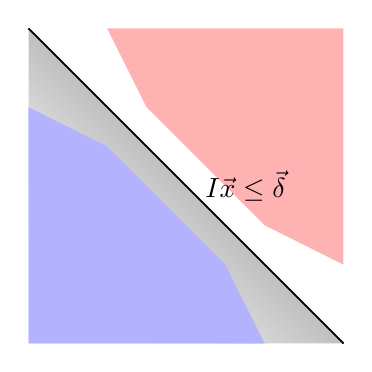
\begin{tikzpicture}[auto, node distance=3cm, semithick]
  \fill[blue!30!white] (0,0) -- (3,0) -- (2.5,1) -- (1,2.5) -- (0,3);
  \fill[red!30!white] (4,4) -- (1,4) -- (1.5,3) -- (3,1.5) -- (4,1);
  \visible<2>{\draw (0,4) to (4,0);}
  \visible<3->{
      \shadedraw[
        shading=axis,
        shading angle=-45,
        draw=none] (0,0) -- (4,0) -- (0,4) -- cycle;
      \fill[blue!30!white] (0,0) -- (3,0) -- (2.5,1) -- (1,2.5) -- (0,3);
      \draw (0,4) to node[right] {\mbox{}\ $I \vec{x} \leq \vec{\delta}$} (4,0);
  }
  \end{tikzpicture}
  \end{figure}
\end{frame}

%\begin{frame}
%  \frametitle{Applications}
%  \begin{itemize}
%  \item Predicate discovery for CEGAR-based model checkers\\
%        for refinement of abstract states.
%  \item Example: CSIsat is the new backend for \\
%        the software model checker \blast{}\footnote{[Henzinger 04] ~ \url{http://mtc.epfl.ch/software-tools/blast/}}:
%    \begin{itemize}
%    \item Improved dependencies and better compilation.
%    \item More comfortable for the user (no need to distinguish between
%      \foci{}\footnote{[McMillan 05] ~  \url{http://www.kenmcmil.com/foci.html}}
%      and \clpprover{}\footnote{[Rybalchenko 07] ~ \url{http://www.mpi-sws.mpg.de/~rybal/clp-prover/}} anymore).
%    \end{itemize}
%  \item Open-source software and freely extendable by others.
%  \end{itemize}
%\end{frame}

\begin{frame}
  \frametitle{Applications}
  \begin{itemize}
  \item Predicate discovery for CEGAR-based model checkers\\
        for refinement of abstract states.
  \item Example: %\csisat{} is the new backend for \\
        \blast{}\footnote{\url{http://mtc.epfl.ch/blast/}} 2.5 is based on \csisat{}:
    \begin{itemize}
      \item<2-> \foci{}\footnote{\url{http://www.kenmcmil.com/foci.html}} for DL + EUF.
      %\item<2-> \foci{}\footnote{[McMillan 05] ~  \url{http://www.kenmcmil.com/foci.html}} for DL + EUF.
      \item<3-> \clpprover{}\footnote{\url{http://www.mpi-sws.mpg.de/~rybal/clp-prover/}} for LA + EUF, but only conjunctions.
      %\item<3-> \clpprover{}\footnote{[Rybalchenko 07] ~ \url{http://www.mpi-sws.mpg.de/~rybal/clp-prover/}} for LA + EUF, but only conjunctions.
      \item<4-> \csisat{} is a new implementation for LA + EUF.
    \end{itemize}
  \item Open-source software and freely extendable by others.
    \begin{itemize}
    \item Total of 7500 lines of code written in Ocaml.
    \item Includes interpolation code and SMT solver.
    \end{itemize}
  \end{itemize}
\end{frame}

\section{How to use \csisat{} ?}
\begin{frame}
  \frametitle{What to give, what to expect}
  \begin{itemize}
  \item Input: $n$ formulae $X_1, \ldots, X_n$ such that
    \begin{equation*}
      \bigwedge_{i=1}^n X_i \models \bot
    \end{equation*}
  \item Output: $n-1$ interpolants such that
    \begin{eqnarray*}
      \bigwedge_{j=1}^i X_j & \models & I_i \\
      I_i \wedge \bigwedge_{j=i+1}^n X_j & \models & \bot
    \end{eqnarray*}
  \end{itemize}
\end{frame}

\begin{frame}[fragile]
  \frametitle{Syntax}
  \begin{itemize}
  \item Formula syntax is very simple and easy to integrate.
  \item \csisat{} supports also \foci{} syntax.
  \end{itemize}
  \vspace*{1cm}
  Example: \textcolor{blue}{$A$: ~ $a = b \wedge b = c$} ~~~~
  \textcolor{red}{$B$: ~ $f(a) \ne f(c)$}
  \begin{verbatim}
  a = b & b = c   ;    not  f(a) = f(c)
  \end{verbatim}
\end{frame}

\begin{frame}
  \frametitle{Example}
  \begin{figure}
  \centering
  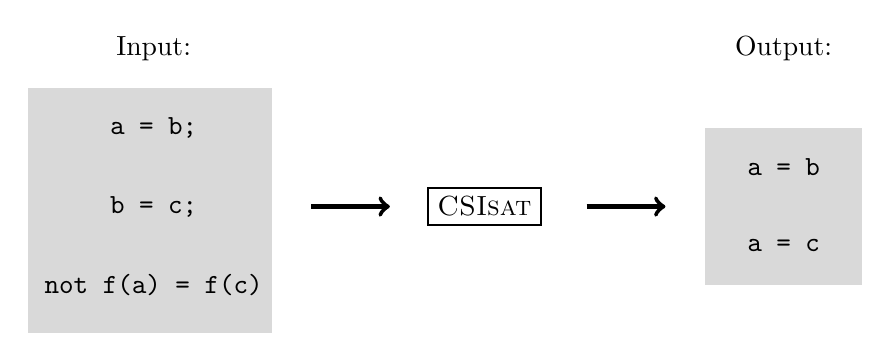
\begin{tikzpicture}[auto, node distance=3cm, semithick]
  \fill[black!15!white] (-1.6,-0.6) rectangle (1.5,2.5);
  \node [draw=none] (in) at (0,3) {Input:};
  \node [draw=none] (x1) at (0,2) {{\tt a = b;}};
  \node [draw=none] (x2) at (0,1) {{\tt b = c;}};
  \node [draw=none] (x3) at (0,0) {{\tt not f(a) = f(c)}};

  \visible<2->{
    \draw [->, ultra thick] (2,1) to (3,1);
    \node [thick,draw] (cs) at (4.2,1) {\csisat{}};
  }
  
  \visible<3->{
    \draw [->, ultra thick] (5.5,1) to (6.5,1);
    \fill[black!15!white] (7,0) rectangle (9,2);
    \node [draw=none] (out) at (8,3) {Output:};
    \node [draw=none] (i1) at (8,1.5) {{\tt a = b}};
    \node [draw=none] (i2) at (8,0.5) {{\tt a = c}};
  }

  \end{tikzpicture}
  \end{figure}
\end{frame}

\section{How \csisat{} works ?}
%\begin{frame}
%  \frametitle{General}
%  \csisat{} combines several known algorithms and provides them as open-source software.
%  \vspace{5pt}
%
%  \begin{tabular}{lcl}
%    Interpolation for EUF & $\rightarrow$ & McMillan 05\\
%    Interpolation for LA & $\rightarrow$ & Rybalchenko et al. 07\\
%    Interpolation using Nelson-Oppen & $\rightarrow$ &   Yorsh et al. 05\\
%     & + & Rybalchenko et al. 07\\
%    Interpolation with a resolution proof & $\rightarrow$  & Yorsh et al. 05
%  \end{tabular}
%
%\end{frame}

\begin{frame}
  \frametitle{Architecture}
  \begin{enumerate}
    \item Generating a resolution proof of unsatisfiability.
    \item<3-> Constructing the interpolant.
  \end{enumerate}

  \begin{figure}
  \centering
  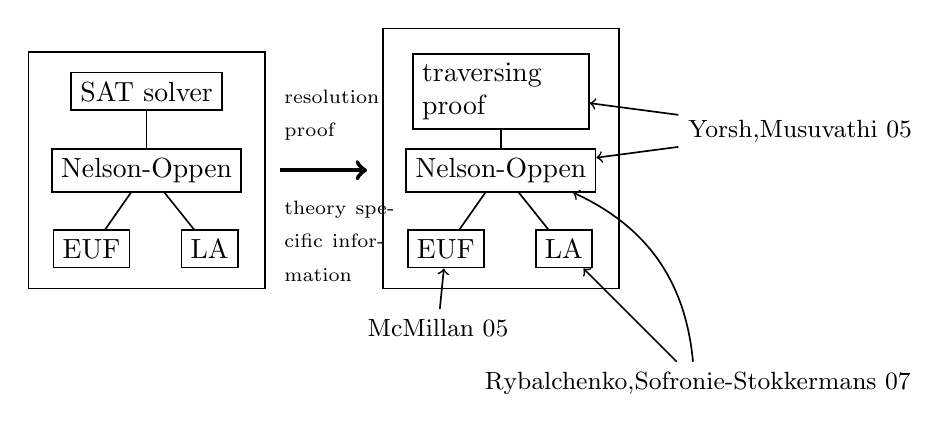
\begin{tikzpicture}[auto, node distance=3cm, semithick]

  \draw (-0.5,-0.5) rectangle (2.5,2.5);
  \node [draw] (sat) at (1,2) {SAT solver};
  \node [draw] (no) at (1,1) {Nelson-Oppen};
  \node [draw] (la) at (1.8,0) {LA};
  \node [draw] (euf) at (0.3,0) {EUF};
  \path (sat) edge (no);
  \path (no) edge (la);
  \path (no) edge (euf);

  \visible<2->{
    \draw [->, ultra thick] (2.7,1) to (3.8,1);
  }
  \visible<2>{
    \node [text width=15mm] (rp) at (3.5,1.7) {\scriptsize resolution proof};
    \node [text width=15mm] (uc) at (3.5,0.1) {\scriptsize theory specific information};
  }
  
  \visible<3->{
    \draw (4,-0.5) rectangle (7,2.8);
    \node [draw,text width=2cm] (trav) at (5.5,2) {traversing proof};
    \node [draw] (no2) at (5.5,1) {Nelson-Oppen};
    \node [draw] (la2) at (6.3,0) {LA};
    \node [draw] (euf2) at (4.8,0) {EUF};
    \path (trav) edge (no2);
    \path (no2) edge (la2);
    \path (no2) edge (euf2);
  }

  \visible<4->{
    \node (yorsh) at (9.3,1.5) {{\small Yorsh,Musuvathi 05}};
    \draw [->] (yorsh) edge  (trav);
  }

  \visible<5->{
    \node (rybal) at (8,-1.7) {{\small Rybalchenko,Sofronie-Stokkermans 07}};
    \draw [->] (yorsh) edge  (no2);
    \draw [->] (rybal) edge [bend right] (no2);
  }
  
  \visible<6->{
    \node (mcmill) at (4.7,-1) {{\small McMillan 05}};
    \draw [->] (mcmill) edge (euf2);
  }
  
  \visible<7->{
    \draw [->] (rybal) edge  (la2);
  }

  \end{tikzpicture}
  \end{figure}
\end{frame}

\section*{Conclusion}
\begin{frame}
  \frametitle{Performance}
  
\begin{figure}
{\footnotesize
\centering
\begin{tabular}{|l|rrrr|}
  \hline
  Program ~~~~~~~ &   \#queries  & ~ \foci{} & ~ \clpprover{}  & \textbf{~\csisat{}}     \\
  \hline
  \hline
  \blast{}\footnote{\url{http://mtc.epfl.ch/blast/}} & & & & \\
  floppy              &   235        & 1.17\,s    &  1.55\,s         & \textbf{0.55\,s}        \\
  cdaudio             &   130        & 0.60\,s    &  0.70\,s         & \textbf{0.26\,s}         \\
  ssh                 &  6881        & 29\,s      & ---              & \textbf{17\,s}         \\
  \hline
  \armc{}\footnote{\url{http://www.mpi-sws.mpg.de/~rybal/armc/}} & & & & \\
  magill      &  9860        & ---        & 30\,s            & \textbf{21\,s}         \\
  \hline
\end{tabular}
}
\end{figure}

\vspace{1cm}
{\footnotesize
Related work: the new version of \mathsat{} [CAV 08] can generate interpolants.
}

\end{frame}

\begin{frame}
  \frametitle{Try it out! }
  \csisat{} is freely available online:
  \begin{itemize}
    \item Project web page:\\ 
          \url{http://www.cs.sfu.ca/~dbeyer/CSIsat}
    \item Sources and bug reports:\\ 
          \url{http://csisat.googlecode.com}
    \item Feedback very welcome!
    \item[]
    \item Questions?
  \end{itemize}
\end{frame}
%-------------------------------------------------------------------------
%\bibliography{../../bib/sw,../../bib/tah}
%\documentclass{beamer}

% To have the citation lists ordered by number.
\usepackage[nocompress]{cite}
\usepackage[utf8]{inputenc}
\usepackage{graphicx}
\usepackage[tight,TABTOPCAP]{subfigure}
\usepackage{amsmath}
\usepackage{amssymb}
\usepackage{amsfonts}
\usepackage{url}

\usepackage{hyperref}

\usepackage{tikz}
\usepackage{color}
\usetikzlibrary{automata,backgrounds,petri}

% Allow more than 70% (default) of a page to be filled by figures (100%).
\renewcommand\topfraction{1.0}

%%%%%%%%%% Tool Names %%%%%%%%%%%%
\newcommand{\csisat}{{\sc CSIsat}}
\newcommand{\blast}{{\sc Blast}}
\newcommand{\armc}{{\sc ARMC}}
\newcommand{\mathsat}{{\sc MathSAT}}
\newcommand{\picosat}{{\sc PicoSAT}}
\newcommand{\clpprover}{{\sc CLPprover}}
\newcommand{\foci}{{\sc Foci}}
\newcommand{\sicstus}{{\sc SICStus Prolog}}
\newcommand{\scala}{\textsc{Scala}}

\mode<presentation>
{
  \usetheme{Warsaw}
  \useoutertheme{mysplit}
}
% Remove the navigation bar
\setbeamertemplate{navigation symbols}{}

\graphicspath{{./imgs/}}

\title[Verifying actors]{Modeling and verifying \scala{} actors}

\AtBeginSection[]
{
  \begin{frame}<beamer>
    \frametitle{Outline}
    \tableofcontents[currentsection]
  \end{frame}
}

\author{ Damien Zufferey}

\institute{
  \'Ecole Polytechnique F\'ed\'erale de Lausanne
}
\date{\today}

%-------------------------------------------------------------------------
\begin{document}

% Title
%\frame[plain]{\titlepage}
\begin{frame}[plain]
%\titlepage
\begin{center}

{\Large
\inserttitle
}

\vspace{10mm}

\insertauthor

\vspace{5mm}

{\footnotesize
\insertinstitute

\vspace{2mm}

\begin{tabular}{ll}
Laboratory: & Models and Theory of Computation\\
Supervisor: & Tom Henzinger\\
Assistant: & Thomas Wies
\end{tabular}
}

\vspace{8mm}
\small
\today
\end{center}
\end{frame}

\section*{Outline}
\begin{frame}
\tableofcontents
\end{frame}

\section{Introduction}

\subsection{Paradigms for concurrency}

\begin{frame}
  \frametitle{Shared memory}
  
  \begin{columns}
  \column{5cm}
  Communication using a memory that every process can access (read and write).

  \column{5cm}
  \centering
  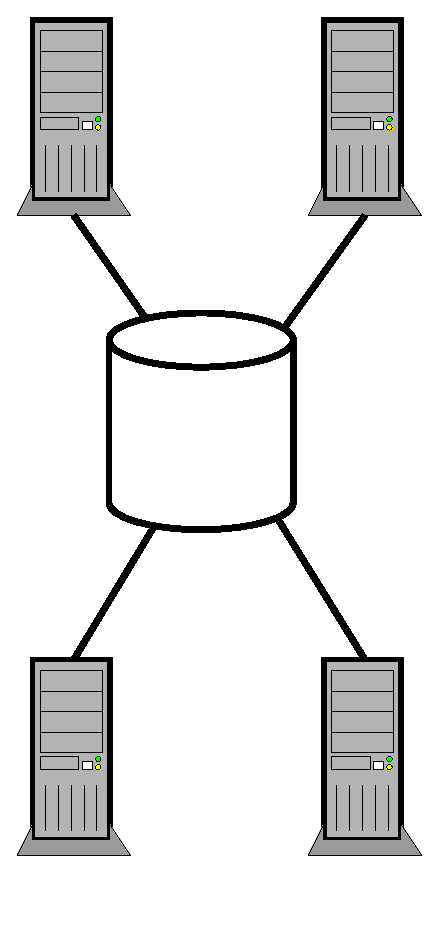
\includegraphics[width=2cm]{shared}
  \end{columns}

  $+$ Fast \\
  $-$ Limited scaling \\
  $-$ Hard to program (deadlocks, races, ...)
\end{frame}

\begin{frame}
  \frametitle{Message passing}
  
  \begin{columns}
  \column{5cm}
  Processes exchange messages.

  \column{5cm}
  \centering
  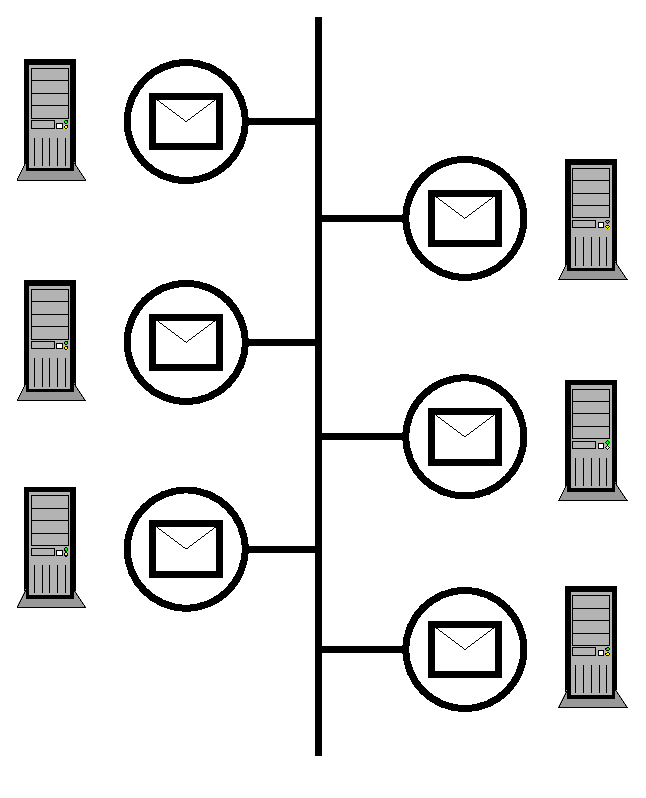
\includegraphics[width=3.5cm]{message}
  \end{columns}

  $+$ Scales well\\
  $-$ Slower \\
  $\sim$ Hard to program (easier than shared memory ?)
\end{frame}

\subsection{Actors in \scala{}}

\begin{frame}[fragile]
  \frametitle{Example (1): scala/docs/examples/actors/pingpong.scala}

  \begin{columns}
    \column{6cm}
{\tiny
\begin{verbatim}
class Ping(count: Int, pong: Actor) extends Actor {
  def act() {
    var pingsLeft = count - 1
    pong ! Ping
    loop {
      react {
        case Pong =>
          if (pingsLeft % 1000 == 0)
            println("Ping: pong")
          if (pingsLeft > 0) {
            pong ! Ping
            pingsLeft -= 1
          } else {
            println("Ping: stop")
            pong ! Stop
            exit()
          }
      }
    }
  }
}
\end{verbatim}
}

    \column{5cm}
{\tiny
\begin{verbatim}
class Pong extends Actor {
  def act() {
    var pongCount = 0
    loop {
      react {
        case Ping =>
          if (pongCount % 1000 == 0)
            println("Pong: ping "+pongCount)
          sender ! Pong
          pongCount += 1
        case Stop =>
          println("Pong: stop")
          exit()
      }
    }
  }
}
\end{verbatim}
}
  \end{columns}
\end{frame}

\begin{frame}[label=cfa]
  \frametitle{Example (2): scala/docs/examples/actors/pingpong.scala}

  \begin{columns}
    \column{5cm}
    \begin{figure}[!ht]
      \centering
      \begin{tikzpicture}[->,auto, node distance=2cm, semithick]
      \node [state,initial] (pi0) {$pi_0$};
      \node [state] (pi1) [below of=pi0] {$pi_1$};
      \node [state] (pi2) [below of=pi1] {$pi_2$};
      \node [state,accepting] (pi3) [right of=pi2] {$pi_3$};
      \path
      (pi0) edge node[left] { pong ! Ping } (pi1)
      (pi1) edge [bend left] node[right] { \_ ? Pong } (pi2)
      (pi2) edge [bend left] node[left] { $pong$ ! Ping } (pi1)
      (pi2) edge [bend right] node[below] { $pong$ ! Stop } (pi3)
      ;
      \end{tikzpicture}
%      \caption{Ping($pong$)}
%      \label{ping}
    \end{figure}

    \column{5cm}
    \begin{figure}[!ht]
      \centering
      \begin{tikzpicture}[->,auto, node distance=2cm, semithick]
      \node [state,initial] (po0) {$po_0$};
      \node [state,accepting] (po1) [below of=po0] {$po_1$};
      \node [state] (po2) [above of=po0] {$po_2$};
      \path
      (po0) edge node[right] { \_ ? Stop } (po1)
      (po0) edge [bend right] node[right] { $X$ ? Ping } (po2)
      (po2) edge [bend right] node[left] { $X$ ! Pong} (po0)
      ;
      \end{tikzpicture}
%      \caption{Pong}
%      \label{pong}
    \end{figure}
  \end{columns}
\end{frame}


\begin{frame}[label=implementation]
  \frametitle{Overview of Analysis}
  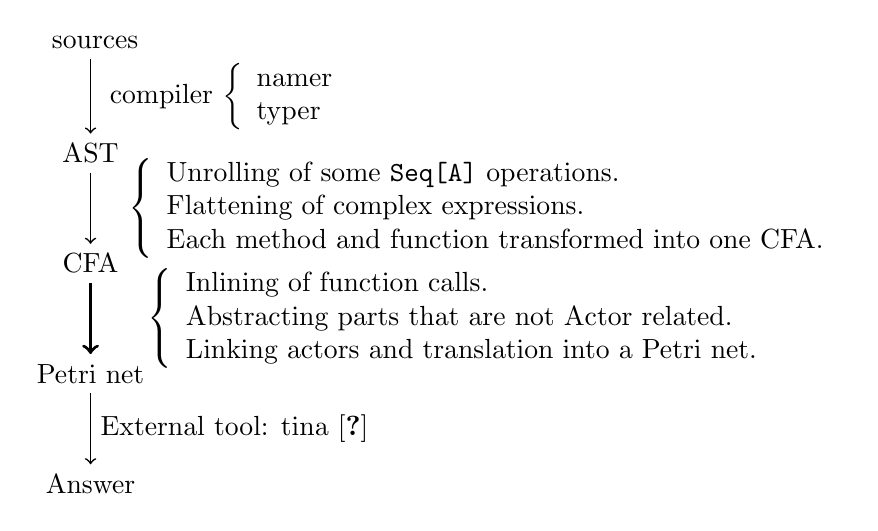
\begin{tikzpicture}[->,auto, node distance=1.4cm, semithick]
    \node (po0) {\scala{} sources};
    \node (po1) [below of=po0] {AST};
    \node (po2) [below of=po1] {CFA};
    \node (po3) [below of=po2] {Petri net};
    \node (po4) [below of=po3] {Answer};
    \path
    (po0) edge node[right] { \scala{} compiler $\left\{ \begin{array}{l} \mbox{namer} \\ \mbox{typer} \end{array} \right.$ } (po1)
    (po1) edge node[right] { ~~ $\left\{ \begin{array}{l}
        \mbox{Unrolling of some \texttt{Seq[A]} operations.} \\
        \mbox{Flattening of complex expressions.} \\
        \mbox{Each method and function transformed into one CFA.}
      \end{array} \right.$ } (po2)
    (po2) edge[very thick] node[right] { ~~~~ $\left\{ \begin{array}{l}
        \mbox{Inlining of function calls.} \\
        \mbox{Abstracting parts that are not Actor related.} \\
        \mbox{Linking actors and translation into a Petri net.} \\
      \end{array} \right.$ } (po3)
    (po3) edge node[right] { External tool: tina\cite{DBLP:conf/qest/BerthomieuV06}} (po4)
    ;
  \end{tikzpicture}
\end{frame}


\section{The Actor Model}

\begin{frame}
  \frametitle{Overview}
  \alt<2>{The \textcolor{red}{Actor Model}\cite{DBLP:conf/ijcai/HewittBS73}}{Object oriented programming}
  uses \emph{\alt<2>{\textcolor{red}{actors}}{objects}} and their interactions
  to build \alt<2>{\textcolor{red}{concurrent} softwares}{software systems}.\\

  \vspace{5pt}

  An \alt<2>{\textcolor{red}{actor}}{object} can:
  \begin{itemize}
  \item receive messages
  \item \alt<2>{\textcolor{red}{create new actors}}{process data}
  \item send messages
  \end{itemize}

  \vspace{10pt}

  \visible<2>{The meaning of messages is not the same in both contexts.}
\end{frame}

\begin{frame}
  \frametitle{Models and decidability}

\begin{tabular}{l|l}
Model & Reachability\\
\hline
\hline
Synchronous & decidable \\
\hline
Asynchronous with queues & undecidable\\
 & \cite{DBLP:journals/jacm/BrandZ83} \\
% many to one or one to one queues & \cite{DBLP:journals/jacm/BrandZ83} \\
\hline
Asynchronous with multisets  & decidable\footnotemark \\
& \cite{DBLP:journals/njc/AmadioM02} \\
\hline
Asynchronous with lossy queues & decidable\footnotemark \\
& \cite{DBLP:journals/iandc/AbdullaJ96} \\
\hline
\end{tabular}

\vspace{20pt}

With recursion, all models are undecidable \cite{DBLP:journals/toplas/Ramalingam00}.

\footnotetext[1]{fixed number of actors}
\footnotetext{undecidable with fair channel \cite{DBLP:journals/iandc/AbdullaJ96a}}

\end{frame}

\begin{frame}
  \frametitle{Chosen model and Assumptions}

  Finite state machines with unordered mailbox (asynchronous).

  \vspace{20pt}

  To preserve decidability, we need to add the following assumptions:
  \begin{itemize}
  \item finite data-types,
  \item no recursion,
  \item no dynamic actor creation.
%  \item static topology.
  \end{itemize}
\end{frame}

\section{$\pi$-calculus and $A\pi$-calculus}

\begin{frame}
\frametitle{What is it ?}
The $\pi$-calculus\cite{DBLP:journals/iandc/MilnerPW92a,DBLP:journals/iandc/MilnerPW92b} is considered to be the $\lambda$-calculus of message-passing concurrency.
It tries to be minimal, but is still able to model complex features:

\begin{itemize}
\item synchronous and asynchronous communication
\item changing topologies
\item dynamic creation of processes and names
\end{itemize}

\vspace{5pt}

The $A\pi$-calculus\cite{DBLP:conf/ecoop/HondaT91,Boudol92asynchronyand} is a restriction of $\pi$-calculus that only allows asynchronous communication.

\end{frame}

\begin{frame}
\frametitle{Grammar}

\begin{tabular}{lclrl}
$P$ & ::= & $x(y).P $                           & input prefix & (receiving messages)\\
    & $|$ & $\overline{x} \langle y \rangle.P $ & output prefix & (sending messages) \\
    & $|$ & $P\;|\;P $                          & parallel composition & \\
    & $|$ & $(\nu x)P $                         & name creation & (names are channels)\\
    & $|$ & $!P $                               & replication & \\
    & $|$ & $0 $                                & unit process & (finished execution)
\end{tabular}

\vspace{1cm}

The only kind of output prefix allowed in $A\pi$-calculus is `$\overline{x} \langle y \rangle.0 $'.

\end{frame}

\begin{frame}
\frametitle{Semantic}

The most important reduction rules:
\begin{equation*}
\overline{x}\langle z \rangle.P \;|\; x(y).Q \rightarrow P \;|\; Q[z/y]
\end{equation*}

\vspace{10pt}

Some congruence rules:
\begin{columns}

\column{5cm}
\begin{itemize}
\item $P\;|\;Q \equiv Q\;|\;P$
\item $P\;|\;0 \equiv P$
\item $(P\;|\;Q)\;|\;R \equiv P\;|\;(Q\;|\;R)$
\end{itemize}

\column{5cm}
\begin{itemize}
\item $(\nu x)(\nu y)P \equiv (\nu y)(\nu x)P$
\item $(\nu x)0 \equiv 0$
\item $!P \equiv P\;|\;!P$
\end{itemize}

\end{columns}
\end{frame}

\begin{frame}
\frametitle{Example}

$
(\nu p_{ing})(\nu p_{ong}) !( \overline{p_{ong}}\langle p_{ing} \rangle. p_{ing}(p_{ong}). 0 )
                     \;|\; !( p_{ong}(p_{ing}). \overline{p_{ing}}\langle p_{ong} \rangle. 0 )
$ \pause \\

\vspace{15pt}

$
(\nu p_{ing})(\nu p_{ong}) !( \overline{p_{ong}}\langle p_{ing} \rangle. p_{ing}(p_{ong}). 0 )
                     \;|\; !( p_{ong}(p_{ing}). \overline{p_{ing}}\langle p_{ong} \rangle. 0 ) $ \\
\hspace{1cm} $       \;|\; \overline{p_{ong}}\langle p_{ing} \rangle. p_{ing}(p_{ong}). 0
                     \;|\; p_{ong}(p_{ing}). \overline{p_{ing}}\langle p_{ong} \rangle. 0 $
\pause \\

\vspace{15pt}

$
(\nu p_{ing})(\nu p_{ong}) !( \overline{p_{ong}}\langle p_{ing} \rangle. p_{ing}(p_{ong}). 0 )
                     \;|\; !( p_{ong}(p_{ing}). \overline{p_{ing}}\langle p_{ong} \rangle. 0 ) $ \\
\hspace{1cm} $       \;|\; p_{ing}(p_{ong}). 0
                     \;|\; \overline{p_{ing}}\langle p_{ong} \rangle. 0 $
\pause \\

\vspace{15pt}

$
(\nu p_{ing})(\nu p_{ong}) !( \overline{p_{ong}}\langle p_{ing} \rangle. p_{ing}(p_{ong}). 0 )
                     \;|\; !( p_{ong}(p_{ing}). \overline{p_{ing}}\langle p_{ong} \rangle. 0 ) $ \\
\hspace{1cm} $       \;|\; 0
                     \;|\; 0 $
\pause \\

\vspace{15pt}

$
(\nu p_{ing})(\nu p_{ong}) !( \overline{p_{ong}}\langle p_{ing} \rangle. p_{ing}(p_{ong}). 0 )
                     \;|\; !( p_{ong}(p_{ing}). \overline{p_{ing}}\langle p_{ong} \rangle. 0 )
$

\end{frame}

\section{Petri nets}

\begin{frame}
\frametitle{Overview}

Petri nets are modeling language for discrete distributed systems.\\

\vspace{10pt}

A Petri net is a directed bipartite graph where the nodes are divided in \emph{places} and \emph{transitions}.\\
Places may contain some tokens, that are consumed and created by transitions.

\end{frame}

\begin{frame}
  \frametitle{Example}

  \begin{columns}
    \column{5cm}
    \begin{figure}[!ht]
      \centering
      \begin{tikzpicture}[->,auto, node distance=2cm, semithick]
      \node [state,color=black!30] (pi0) {$pi_0$};
      \node [state,initial] (pi1) [below of=pi0] {$pi_1$};
      \node [state] (pi2) [below of=pi1] {$pi_2$};
      \node [state,accepting,color=black!30] (pi3) [right of=pi2] {$pi_3$};
      \path
      (pi0) edge [color=black!30] node[left] { pong ! Ping } (pi1)
      (pi1) edge [bend left] node[right] { \_ ? Pong } (pi2)
      (pi2) edge [bend left] node[left] { $pong$ ! Ping } (pi1)
      (pi2) edge [bend right,color=black!30] node[below] { $pong$ ! Stop } (pi3)
      ;
      \end{tikzpicture}
    \end{figure}

    \column{5cm}
    \begin{figure}[!ht]
      \centering
      \begin{tikzpicture}[->,auto, node distance=2cm, semithick]
      \node [state,initial] (po0) {$po_0$};
      \node [state,accepting,color=black!30] (po1) [below of=po0] {$po_1$};
      \node [state] (po2) [above of=po0] {$po_2$};
      \path
      (po0) edge [color=black!30] node[right] { \_ ? Stop } (po1)
      (po0) edge [bend right] node[right] { $X$ ? Ping } (po2)
      (po2) edge [bend right] node[left] { $X$ ! Pong} (po0)
      ;
      \end{tikzpicture}
    \end{figure}
  \end{columns}
\end{frame}


\begin{frame}
\frametitle{Example}
\begin{figure}[!ht]
  \centering
  \begin{tikzpicture}[auto, node distance=2cm, semithick]

  \node (label1) at (-4,3) {ping state};
  \node (label2) at ( 0,3) {mailboxes};
  \node (label3) at ( 4,3) {pong state};
  \draw[dashed] (-1.5,-1) -- (-1.5,3);
  \draw[dashed] (1.5,-1) -- (1.5,3);

  \alt<1,5>{
  \node [place,fill=red!18] (ping) at (0,0) {};
  \node [place,tokens=1,fill=blue!18] (pong) [above of= ping] {};

  \node [transition,very thick] (pongCatch) [right of= pong] {};
  \node [transition] (pongSend)  [below of= pongCatch] {};
  \node [place,tokens=1,fill=blue!30] (po0) [right of= pongCatch] {};
  \node [place,fill=blue!30] (po1) [below of= po0] {};
  
  \node [transition] (pingCatch) [left of = ping] {};
  \node [transition] (pingSend) [above of= pingCatch] {};
  \node [place,tokens=1,fill=red!30] (pi0) [left of= pingCatch] {};
  \node [place,fill=red!30] (pi1) [above of= pi0] {};
  }{
  \alt<2>{
  \node [place,fill=red!18] (ping) at (0,0) {};
  \node [place,fill=blue!18] (pong) [above of= ping] {};

  \node [transition] (pongCatch) [right of= pong] {};
  \node [transition,very thick] (pongSend)  [below of= pongCatch] {};
  \node [place,fill=blue!30] (po0) [right of= pongCatch] {};
  \node [place,tokens=1,fill=blue!30] (po1) [below of= po0] {};
  
  \node [transition] (pingCatch) [left of = ping] {};
  \node [transition] (pingSend) [above of= pingCatch] {};
  \node [place,tokens=1,fill=red!30] (pi0) [left of= pingCatch] {};
  \node [place,fill=red!30] (pi1) [above of= pi0] {};
  }{
  \alt<3>{
  \node [place,tokens=1,fill=red!18] (ping) at (0,0) {};
  \node [place,fill=blue!18] (pong) [above of= ping] {};

  \node [transition] (pongCatch) [right of= pong] {};
  \node [transition] (pongSend)  [below of= pongCatch] {};
  \node [place,tokens=1,fill=blue!30] (po0) [right of= pongCatch] {};
  \node [place,fill=blue!30] (po1) [below of= po0] {};
  
  \node [transition,very thick] (pingCatch) [left of = ping] {};
  \node [transition] (pingSend) [above of= pingCatch] {};
  \node [place,tokens=1,fill=red!30] (pi0) [left of= pingCatch] {};
  \node [place,fill=red!30] (pi1) [above of= pi0] {};
  }{
  \node [place,fill=red!18] (ping) at (0,0) {};
  \node [place,fill=blue!18] (pong) [above of= ping] {};

  \node [transition] (pongCatch) [right of= pong] {};
  \node [transition] (pongSend)  [below of= pongCatch] {};
  \node [place,tokens=1,fill=blue!30] (po0) [right of= pongCatch] {};
  \node [place,fill=blue!30] (po1) [below of= po0] {};
  
  \node [transition] (pingCatch) [left of = ping] {};
  \node [transition,very thick] (pingSend) [above of= pingCatch] {};
  \node [place,fill=red!30] (pi0) [left of= pingCatch] {};
  \node [place,tokens=1,fill=red!30] (pi1) [above of= pi0] {};
  }
  }
  }
  \path
    (pingCatch) edge [pre] (pi0)
                edge [pre] (ping)
                edge [post] (pi1)
    (pingSend)  edge [pre] (pi1)
                edge [post] (pi0)
                edge [post] (pong)
    (pongCatch) edge [pre] (po0)
                edge [pre] (pong)
                edge [post] (po1)
    (pongSend)  edge [pre] (po1)
                edge [post] (po0)
                edge [post] (ping)
  ;

  \end{tikzpicture}
\end{figure}
\end{frame}

\begin{frame}
\frametitle{Decidability}
Problems like covering, liveness of transitions, reachability for Petri net are decidable, but very expensive (EXPSPACE-hard \cite{DBLP:conf/stoc/CardozaLM76}).\\

\vspace{20pt}

A survey for Petri nets decidability and complexity for different problems can be found at \cite{DBLP:journals/eik/EsparzaN94}.
\end{frame}

\section*{Conclusion}

\begin{frame}
  \frametitle{Summary}
  \begin{itemize}
  \item Safety properties are decidable for a subset of the Actor model.
  \item The theoretical justification lies in the $A\pi$-calculus.
  \item Petri nets are used for back-end computations.
  \item The Implementation is done up to the translation into Petri nets.
  \end{itemize}
\end{frame}

\againframe{implementation}

\begin{frame}
  \frametitle{Further Work}
  One limitation is the \textbf{features} that are supported.\\
  Adding more features means going toward (and beyond) the frontier of decidability.

  \vspace{30pt}

  Another limitation of this verification method is its \textbf{complexity}.\\
  $\Rightarrow$ Compositional verification.
\end{frame}

\begin{frame}
  \frametitle{}
  {\tiny
  %\bibliographystyle{annotate}
  %\bibliographystyle{plainnat}
  \bibliographystyle{cell}
  %\bibliographystyle{abbrvnat}
  \bibliography{b}
  }
\end{frame}

\end{document}


\end{document}
